\documentclass[lang=cn,newtx,10pt,scheme=chinese]{elegantbook}

\title{\LaTeX{} 随笔}
\subtitle{Elegant\LaTeX{} 入门之作}

\author{SummerSong}
% \institute{}
\renewcommand{\today}{\number\year 年 \number\month 月 \number\day 日}
\date{\today}
% \version{4.5}
% \bioinfo{自定义}{信息}

% \extrainfo{注意:本模板自 2023 年 1 月 1 日开始,不再更新和维护!}

\setcounter{tocdepth}{3}

\logo{logo-blue.png}
\cover{cover.jpg}

% 本文档命令
\usepackage{array}
\newcommand{\ccr}[1]{\makecell{{\color{#1}\rule{1cm}{1cm}}}}

% 修改标题页的橙色带
\definecolor{customcolor}{RGB}{32,178,170}
\colorlet{coverlinecolor}{customcolor}
\usepackage{cprotect}

% 自定义qaq命令
\newcommand{\qaq}[1]{\textcolor{red}{\kaishu\large #1}}
% 代码左右展示
\usepackage{array,tabularx}
\usepackage{verbatim}
\usepackage{xeCJKfntef}
\newbox\savedlines
\newtoks\savedtokens
\makeatletter
\def\codeshow{%
\global\savedtokens={}%
\def\verbatim@processline{%
  {\setbox0=\hbox{\the\verbatim@line}%
      \hsize=\wd0
      \the\verbatim@line\par}%
  \global\savedtokens=\expandafter{\the\expandafter\savedtokens\the\verbatim@line^^J}}%
\@tempswatrue
\setbox0=\vbox\bgroup\parskip=0pt\topsep=0pt\partopsep=0pt
\verbatim}
\def\endcodeshow{\endverbatim%
  \unskip\setbox0=\lastbox\egroup
  \global\setbox\savedlines=\box0
  \addvspace{1em}\par\noindent%
  \colorbox{lightgray}{%
    \begin{minipage}{.55\textwidth}{\usebox\savedlines}\end{minipage}}%
  \hfill\fbox{\parbox{.40\textwidth}%
    {\scantokens\expandafter{\the\savedtokens\unskip\endinput}}}%
  \par\addvspace{1em}}
\makeatother

% 完全引用
\usepackage{cleveref}

% 定义交叉引用格式
\newcommand*{\fullref}[1]{第 \ref{#1} \namecref{#1} \nameref{#1} }
\crefname{theorem}{定理}{定理}
\crefname{lemma}{引理}{引理}
\crefname{definition}{定义}{定义}
\crefname{figure}{图}{图}
\crefname{table}{表}{表}
\crefname{algorithm}{算法}{算法}
\crefname{chapter}{章}{章}
\crefname{section}{节}{节}
\crefname{subsection}{条}{条}


\begin{document}

\maketitle
\frontmatter
\tableofcontents
\mainmatter

%正文
% !TEX root = ../latexnote.tex
\chapter*{版本更新历史}
\addcontentsline{toc}{chapter}{版本更新历史}
\datechange{2024/04/10}{动笔}
\begin{change}
  \item 开始记录
  \item 添加\fullref{subsec:not-in-order}
  \item 添加\fullref{chap:latex}内容
\end{change}

\datechange{2024/04/17}{完成\fullref{chap:format}}
\begin{change}
  \item 添加\fullref{chap:format}内容
\end{change}

\datechange{2024/04/18}{完成\fullref{chap:text}、\fullref{chap:figure}}
\begin{change}
  \item 添加\fullref{chap:text}内容
  \item 添加\fullref{chap:figure}内容
\end{change}

\datechange{2024/04/23}{完成\fullref{chap:table}、\fullref{chap:math}}
\begin{change}
  \item 添加\fullref{chap:table}内容
  \item 调整章节顺序
  \item 添加\fullref{chap:math}内容
\end{change}

\datechange{2024/05/08}{添加\fullref{chap:refinfor}部分}
\begin{change}
  \item 添加了三个参考资料
\end{change}

\datechange{2024/05/09}{添加\fullref{chap:ref}部分问题}
\begin{change}
  \item 添加\fullref{subsec:year-only}
  \item 添加\fullref{subsec:et-al-italic}
\end{change}

\datechange{2024/05/15}{添加\fullref{subsec:beamer-ref-break}部分问题}
\begin{change}
  \item 添加\fullref{subsec:beamer-ref-break}
\end{change}

\datechange{2024/05/21}{添加\fullref{subsec:longtable-arydshln-conflict}部分问题}
\begin{change}
  \item 添加\fullref{subsec:longtable-arydshln-conflict}
\end{change}

\datechange{2024/06/02}{添加\fullref{subsec:texlive_cn_username}部分问题}
\begin{change}
  \item 添加\fullref{subsec:texlive_cn_username}
\end{change}

\datechange{2024/06/03}{添加\fullref{subsec:pifontconflict}部分问题}
\begin{change}
  \item 添加\fullref{subsec:pifontconflict}
\end{change}

\datechange{2024/06/08}{添加\fullref{subsec:lstlistings}内容}
\begin{change}
  \item 添加\fullref{subsec:lstlistings}
\end{change}

\datechange{2024/06/11}{添加\fullref{subsec:cline-undefined-control-sequence-error}及\fullref{subsec:multirow-center}内容}
\begin{change}
  \item 添加\fullref{subsec:cline-undefined-control-sequence-error}
  \item 添加\fullref{subsec:multirow-center}
\end{change}

% !TEX root = ../latexnote.tex
\chapter{\LaTeX{} 基础}\label{chap:latex}
\section{\LaTeX{} 家族}\label{sec:latexfamily}
本节介绍一下各种名词,这里主要引用一篇知乎文章:\href{https://zhuanlan.zhihu.com/p/248669482}{TeX 家族(TeX, XeTeX, LuaTeX,XeLaTeX …看完这篇就懂了)},加之个人理解。
\elegantnewtheorem{explain}{}{defstyle}
\begin{explain*}{引擎}
    引擎是真正干活的程序。引擎的基本功能就是解释TeX语法,把字排成行,把行排成页,涉及到断字、断行、分页等算法。最原始的引擎是TeX。
    \begin{itemize}
        \item TeX:1978年由Donald Erwin Knuth(高德纳)开发。是后来大部分TeX相关的基础。其生成dvi文件,然后经由其他程序转换为pdf文件.
        \item pdfTeX:Tex语言的又一个实现,将TeX代码直接编译成PDF文件。
        \item XeTeX:TeX 语言的新的实现,支持 Unicode 编码和直接访问操作系统字体。
        \item LuaTeX:TeX 语言的一个完整的有扩展的实现。LuaTeX支持Unicode、系统字体和内嵌语言扩展,能直接输出PDF格式文件,也可以仍然输出 DVI 格式。
    \end{itemize}

    \bf{我的理解:TeX相当于汇编语言。}
\end{explain*}

\begin{explain*}[格式]
    TeX语言本身只有300个命令,晦涩难懂,只适合非正常的人类。一个简单的符号可能就需要多个命令来实现,可以将这些最基本的命令封装起来做个简写(宏)以实现特殊的目的。一堆简写的合集就构成了格式。格式可以与不同的引擎相结合。
    \begin{itemize}
        \item Plain TeX:由Don Knuth提供的最小的宏集合。
        \item LaTeX:更易于使用的宏集,最常见的一种格式。
        \item ConTeXt:另一种常见的格式。
    \end{itemize}


    \bf{我的理解:格式就是C语言等高级语言}
\end{explain*}

\begin{explain*}[编译命令]
    是实际调用的、结合了引擎和格式的命令。如 \lstinline{xelatex} 命令是结合  XeTeX 引擎和    LaTeX 格式的一个编译命令。
\end{explain*}

\begin{explain*}[宏包]
    一些辅助文件,在LaTeX中叫做packages,在ConTeXt中叫做modules。在LaTeX格式中,导言区的usepackage的作用就是引入各种宏包。宏包其实也是一堆基本的TeX命令的集合,只是其不够全,所以称之为宏包而不是格式。

    \bf{我的理解:宏包类似python的库,里面有封装好的函数}
\end{explain*}

\begin{explain*}[发行版]
    一个完整的TeX需要最基本的TeX引擎、格式支持、各种辅助宏包、一些转换程序、GUI、编辑器、文档查看器等等。通过选择不同的组合就构成了不同的发行版。
    \begin{itemize}
        \item TeX Live:支持Linux,Windows,Mac OS
        \item MiKTeX:只支持Windows
        \item CTeX:CTeX基于MiKTeX,并加入了中文的支持,只支持Windows。同时CTEX是一个网站,ctex是可以很好支持中文的宏包。
    \end{itemize}

    \bf{我的理解:IDE?}
\end{explain*}

\section{\LaTeX{} 安装}\label{sec:latexinstall}
参考\href{https://summersong.top/post/1f879cd9.html}{TexLive+VScode+SumatraPDF配置LaTex编辑环境}

\subsection{用户名为中文安装Texlive失败}\label{subsec:texlive_cn_username}
\qaq{问题:}在使用 GUI 界面安装时, 出现的错误形如图\ref{fig:failuregui}
\begin{figure}[!h]
    \centering
    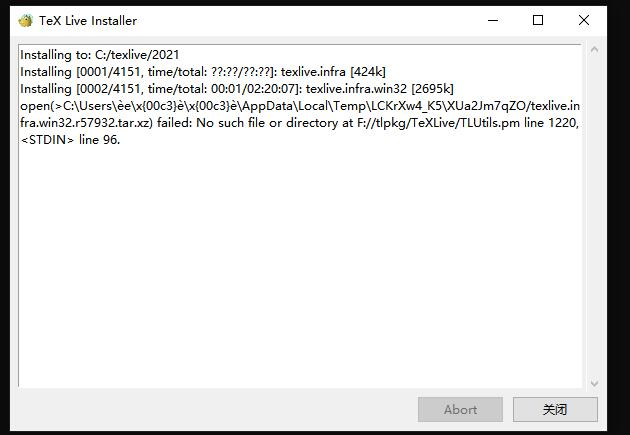
\includegraphics[width=0.8\textwidth]{figure/chap-basic/failuregui.jpg}
    \caption{Texlive 安装错误}\label{fig:failuregui}
\end{figure}

\qaq{解决方法:}参考\href{https://syvshc.github.io/2021-04-07-illegal-temp-cause-tlinstall-failure/}{Windows 不合法的缓存路径导致 TeX Live 安装失败},建议临时修改\lstinline{TEMP}与\lstinline{TMP}环境变量的值。在cmd中输入以下命令:
\begin{lstlisting}
    mkdir C:\temp
    set TEMP=C:\temp
    set TMP=C:\temp
\end{lstlisting}

然后运行安装脚本。

\section{\LaTeX{} 命令和代码结构}\label{sec:latexstructure}
\subsection{最短的\LaTeX{}代码}\label{subsec:shortlatexcode}
\begin{lstlisting}
\documentclass{article}
\begin{document}
Hello, \LaTeX{}!
\end{document}
\end{lstlisting}

上述代码是\LaTeX{} 排版的最短代码。下面简单介绍\LaTeX{}命令和代码的结构。

\subsection{\LaTeX{}命令和环境}\label{subsec:latexcommands}

\LaTeX{}命令以反斜杠 \hspace{0.2em}\textbackslash\hspace{0.2em} 开头,后面跟一串字母,如\lstinline{\LaTeX}。它们以任意非字母符号为界限。

要注意\LaTeX{} 命令是对大小写敏感的,比如输入 \lstinline{\LaTeX} 命令可以生成错落有致的 \LaTeX{} 字母组合,但输入 \lstinline{\Latex} 或者 \lstinline{\LaTex} 什么都得不到,还会报错;它们与 \lstinline{\LaTeX} 是不同的命令。

一些 \LaTeX{} 命令可以接收一些参数,参数的内容会影响命令的效果。\LaTeX{} 的参数分为可选参数和必选参数。可选参数以方括号 [] 包裹;必选参数一般以花括号 \{\} 包裹。还有些命令可以带一个星号*,带星号和不带星号的命令效果有一定差异,一般是带不带编号,比如章节标题。

\LaTeX{} 中还包括{\bf 环境},用以令一些效果在局部生效,或是生成特殊的文档元素。\LaTeX{} 环境的用法为一对命令 \lstinline{\begin} 和 \lstinline{\end}:
\begin{lstlisting}
\begin{环境名称}[可选参数]{必选参数}
    内容
\end{环境名称}
\end{lstlisting}

有些命令(如 \lstinline{\bfseries})会对其后所有内容产生作用。若要限制其作用范围,则需要使用{\bf 分组}。\LaTeX{} 使用一对花括号
\{\} 作为分组,在分组中使用的命令被限制在分组内,不会影响到分组外的内容。

\subsection{\LaTeX{}源代码结构}\label{subsec:latexsourcestructure}
LATEX 源代码以一个 \lstinline{\documentclass} 命令作为开头,它指定了文档使用的文档类。document 环境当中的内容是文档正文。

在 \lstinline{\documentclass} 和 \lstinline|\begin{document}|之间的位置称为{\bf 导言区}。在导言区中常会使用\lstinline{\usepackage} 命令调用{\bf 宏包},还会进行文档的全局设置。

\begin{lstlisting}

    \documentclass{...} % ...为某文档类,比如artile、book、report等
    % 导言区 
    \usepackage{ctex} %加载 ctex 宏包
    \begin{document}
    这里是正文。
    \end{document}
    %此后内容被忽略。

\end{lstlisting}

在正文区中,一般会包含一些文本、公式、图表、表格等内容。

\section{\LaTeX{} 文档类和宏包}\label{sec:latexclasses}
\subsection{\LaTeX{} 文档类}\label{subsec:latexdocclass}
文档类规定了 \LaTeX{} 源代码所要生成的文档的性质——普通文章、书籍、演示文稿、个人简历等等。\LaTeX{}源代码的开头须用\lstinline{\documentclass} 指定文档类:

\begin{lstlisting}
\documentclass[可选参数]{文档类名称}
\end{lstlisting}

文档类如\LaTeX{}提供的 article、report、book,在其基础上派生的一些文档类,如支持中文排版的 ctexart、ctexrep、ctexbook,或者有其它功能的一些文档类,如 moderncv、beamer 等。\LaTeX{} 提供的基础文档类见表\ref{tab:latex_doc_class},其中前三个习惯上称为“标准文档
类”。

\begin{table}[!h]
    \centering
    \caption{\LaTeX{} 文档类}
    \label{tab:latex_doc_class}
    \begin{tabular}{ll}
        \toprule
        类别      & 说明   \\
        \midrule
        article & 普通文章 \\
        book    & 书籍   \\
        report  & 报告   \\
        \hline
        letter  & 信件   \\
        slides  & 幻灯片  \\
        beamer  & 幻灯片  \\
        memoir  & 书籍类  \\
        acmart  & 科技论文 \\
        \bottomrule
    \end{tabular}
\end{table}

{\bf 可选参数}为文档类指定选项,以全局地规定一些排版的参数,如字号、纸张大小、单双面等等。比如调用 \lstinline{article} 文档类排版文章,指定纸张为 A4 大小,基本字号为 11pt,双面排版:
\begin{lstlisting}
\documentclass[11pt,a4paper,twoside]{article}
\end{lstlisting}

\subsection{\LaTeX{} 宏包}\label{subsec:latexpackage}
在使用 \LaTeX{} 时,时常需要依赖一些扩展来增强或补充\LaTeX{}的功能,比如排版复杂的表格、插入图片、增加颜色甚至超链接等等。这些扩展称为宏包。调用宏包的方法非常类似调用文档类的方法:
\begin{lstlisting}
\usepackage[可选参数]{宏包名称}
\end{lstlisting}
\lstinline{\usepackage} 可以一次性调用多个宏包:

\begin{lstlisting}
    % 一次性调用三个排版表格常用的宏包
    \usepackage{tabularx, makecell, multirow}
\end{lstlisting}

\section{\LaTeX{} 使用到的文件类型}\label{sec:latexfiletypes}

除了源代码文件 \lstinline{.tex} 以外,我们在使用 \LaTeX{} 时还可能接触到各种格式的文件。本节简单介绍一下在使用 \LaTeX{} 时能够经常见到的文件。

每个宏包和文档类都是带特定扩展名的文件,除此之外也有一些文件出现于 \LaTeX{} 模板中:

\begin{itemize}
    \item \lstinline{.sty} 宏包文件。宏包的名称与文件名一致。
    \item \lstinline{.cls} 文档类文件。文档类名称与文件名一致。
    \item \lstinline{.bib} BibTeX 参考文献数据库文件。
    \item \lstinline{.bst} BibTeX 用到的参考文献格式模板。
\end{itemize}

\LaTeX{} 在编译过程中除了生成 .dvi 或 .pdf 格式的文档外,还可能会生成相当多的辅助文件和日志。一些功能如交叉引用、参考文献、目录、索引等,需要先通过编译生成辅助文件,然后再次编译时读入辅助文件得到正确的结果,所以复杂的 \LaTeX{} 源代码可能要编译多次:

\begin{itemize}
    \item \lstinline{.log} 排版引擎生成的日志文件,供排查错误使用。
    \item \lstinline{.aux} \LaTeX{} 生成的主辅助文件,记录交叉引用、目录、参考文献的引用等。
    \item \lstinline{.toc} \LaTeX{} 生成的目录记录文件。
    \item \lstinline{.lof} \LaTeX{} 生成的图片目录记录文件。
    \item \lstinline{.lot} \LaTeX{} 生成的表格目录记录文件。
    \item \lstinline{.bbl} BibTeX 生成的参考文献记录文件。
    \item \lstinline{.blg} BibTeX 生成的日志文件。
    \item \lstinline{.idx} \LaTeX{} 生成的供 makeindex 处理的索引记录文件。
    \item \lstinline{.ind} makeindex 处理 .idx 生成的用于排版的格式化索引文件。
    \item \lstinline{.ilg} makeindex 生成的日志文件。
    \item \lstinline{.out} hyperref 宏包生成的 PDF 书签记录文件。
\end{itemize}

\section{\LaTeX{} 文件组织方式}\label{sec:latexfileorganization}

编写长篇文档时,例如当编写书籍、毕业论文时,单个源文件会使修改、校对变得十分困难。将源文件分割成若干个文件,例如将每章内容单独写在一个文件中,会大大简化修改和校对的工作。

\LaTeX{} 提供了命令 \lstinline{\include} 用来在源代码里插入文件:

\begin{lstlisting}
\include{chapter1}
\include{chapter2}
\include{chapter3}
\end{lstlisting}

需要注意的是,\lstinline{\include} 命令在读入新的文件之前会另起一页。有的时候我们不需要这样,则用\lstinline{\input} 命令,它仅仅只是将文件里面的内容插入到当前位置。

当导言区内容较多时,常常将其单独放置在一个 \lstinline{.tex} 文件中,再用 \lstinline{\input} 命令插入。复杂的图、表、代码等也会用类似的手段处理。

LATEX 还提供了一个 \lstinline{\includeonly} 命令来组织文件,用于导言区,指定只载入某些文件。导言区使用了 \lstinline{\includeonly} 后,正文中不在其列表范围的 \lstinline{\include}命令不会起效:
\begin{lstlisting}
\includeonly{chapter1,chapter3}
\end{lstlisting}


% !TEX root = ../latexnote.tex
\chapter{版面和格式}\label{chap:format}



\section{字体设置}\label{sec:font}
\subsection{使用中文}\label{subsec:chinese}
使用中文需要导入ctex宏包。
\begin{lstlisting}
\usepackage{ctex}
\end{lstlisting}

\subsection{全局字体设置}\label{subsec:global}

\begin{lstlisting}
  \setmainfont{Times New Roman}	%仅对西文起作用,需要fontspec宏包
  \setCJKmainfont{SimSun}			%仅对中文起作用
\end{lstlisting}

\subsection{局部字体设置}\label{subsec:local}

\begin{lstlisting}
  \setCJKfamilyfont{zhsong}{FZShuSong-Z01}
  \newcommand*{\songti}{\CJKfamily{zhsong}}
\end{lstlisting}

可以使用\lstinline{\songti}命令来调用宋体字体。

\subsection{文字装饰}\label{subsec:decor}

\LaTeX{} 提供\lstinline{\underline}命令设置下划线。

\begin{codeshow}
  \underline{underlined text}
\end{codeshow}

\lstinline{\underline}命令提供的下划线样式不够灵活,ulem或CJKfntef宏包提供了更灵活的下划线命令,CJKfntef宏包对中文支持更好。

\begin{codeshow}
  \CJKunderdot{important 非常重要}\\
  \CJKunderline{notice 注意}\\
  \CJKunderdblline{urgent 必须}\\
  \CJKunderwave{prompt 提示}\\
  \CJKsout{wrong 错误}\\
  \CJKxout{removed 删除}
\end{codeshow}

\section{分栏}\label{sec:columns}

\LaTeX{} 支持简单的单栏或双栏排版。标准文档类的全局选项 onecolumn、twocolumn 可控制全文分单栏或双栏排版。LATEX 也提供了切换单/双栏排版的命令:

\begin{lstlisting}
\onecolumn
\twocolumn
\end{lstlisting}

切换单/双栏排版时总是会另起一页(\lstinline{\clearpage})。在双栏模式下使用 \lstinline{\newpage} 会换栏而不是换页;\lstinline{\clearpage} 则能够换页。

使用multicol宏包可以实现多栏排版。并且切换不会另起一页。

\begin{lstlisting}
\usepackage{multicol}
\begin{multicols}{2}
  ...
\end{multicols}
\end{lstlisting}

\section{断行、断页、断词}\label{sec:break}

\begin{lstlisting}
\\[length] % \\可以带可选参数length,用于在断行处添加垂直间距,可以在表格公式等地方使用
\newline %不带可选参数,只能用于文本段落中

\newpage %双栏模式下另起一栏,单栏模式下另起一页
\clearpage %单栏、双栏模式下都另起一页
\end{lstlisting}

如果 \LaTeX{} 遇到了很长的英文单词,仅在单词之间的“空格”处断行无法生成疏密程度匀称的段落时,就会考虑从单词中间断开。对于绝大多数单词,\LaTeX{} 能够找到合适的断词位置,在断开的行尾加上连字符\lstinline{-}。如果一些单词没能自动断词,我们可以在单词内手动使用 \lstinline{\-} 命令指定断词的位置:

\begin{codeshow}
  I think this is: su\-per\-cal\-%
  i\-frag\-i\-lis\-tic\-ex\-pi\-%
  al\-i\-do\-ciousu\-per\-cal\-%
  i\-frag\-i\-lis\-tic\.
\end{codeshow}

\section{空格和分段}\label{sec:space}
\LaTeX{} 源代码中,空格键和 Tab 键输入的空白字符视为“空格”。连续的若干个空白字符视为一个空格。一行开头的空格忽略不计。

行末的换行符视为一个空格;但连续两个换行符,也就是空行,会将文字分段。多个空行被视为一个空行。也可以在行末使用 \lstinline{\par} 命令分段。

\begin{codeshow}
  This is a new paragraph. Text text text
  text text   text text text text text text.

  This is a new paragraph.\par
  This is a new paragraph.
\end{codeshow}

\section{注释}\label{sec:comment}
LATEX 用 \% 字符作为注释。在这个字符之后直到行末,所有的字符都被忽略,行末的换行符也不引入空格。

\begin{codeshow}
  This is an % short comment
  % ---
  % Long and organized
  % comments
  % ---
  example: Comments do not bre%
  ak a word.
\end{codeshow}

\section{特殊字符}\label{sec:special}

以下字符在 LATEX 里有特殊用途,如 \% 表示注释,\$、\^{}、\_ 等用于排版数学公式,\& 用于排版表格,等等。直接输入这些字符得不到对应的符号,还往往会出错:

\begin{lstlisting}
  # $ % & { } _ ^ ~ \
\end{lstlisting}

如果想要输入以上符号,需要使用以下带反斜线的形式输入,类似编程语言里的“转义”符号:
\begin{lstlisting}
  \# \$ \% \& \{ \} \_
  \^{} \~{} \textbackslash
\end{lstlisting}

\section{问题}\label{sec:qa}
\subsection{双面空白页}\label{subsec:blankpage}
\qaq{问题:}采用\lstinline{twoside}文档类,使用\lstinline{\cleardoublepage}设置双面空白页,如何去除空白页?

\qaq{解决方法:}在所有\lstinline{\cleardoublepage}之前添加\lstinline{\let\cleardoublepage\clearpage}。
% !TEX root = ../latexnote.tex
\chapter{正文工具}\label{chap:text}
\section{章节}\label{sec:section}

一篇结构化的、条理清晰文档一定是层次分明的,通过不同的命令分割为章、节、小节。三个标准文档类 article、report 和 book\footnote{千万注意是标准文档类,其它文档类,如果不是从标准文档类衍生而来,很可能没有定义或只定义了一部分命令}提供了划分章节的命令:
\begin{lstlisting}
\chapter{章名}
\section{节名}
\subsection{小节名}
\subsubsection{}
\paragraph{}
\subparagraph{}
\end{lstlisting}

带星号版本不进行编号,也不生成目录项和页眉页脚。

\section{目录}\label{sec:toc}

在合适部分添加:
\begin{lstlisting}
\tableofcontents
\end{lstlisting}

上述命令会生成目录,标题默认是“Contents”,可通过下列命令更改:
\begin{lstlisting}
\renewcommand{\contentsname}{目录}
\end{lstlisting}

要正确生成目录项,一般需要编译两次源代码。

如果要将使用\lstinline|\chapter*{}|命令的章节加入目录中,需要使用:
\begin{lstlisting}
\addcontentsline{toc}{level}{title} %level为chapter,section等,title为章节名
\end{lstlisting}

\section{页眉页脚}\label{sec:headerfooter}
\subsection{基本的页眉页脚样式}\label{subsec:basic}

\LaTeX{} 中提供了命令 \lstinline{pagestyle} 来修改页眉页脚的样式:
\begin{lstlisting}
    \pagestyle{page-style}
\end{lstlisting}

命令 \lstinline{thispagestyle} 只影响当页的页眉页脚样式:
\begin{lstlisting}
    \thispagestyle{page-style}
\end{lstlisting}

\lstinline{page-style} 参数为样式的名称,在 \LaTeX{} 里预定义了四类样式,见表 \ref{tbl:pagestyle}。

\begin{table}[htp]
    \centering
    \renewcommand\arraystretch{1.5}
    \caption{\LaTeX{} 预定义的页眉页脚样式}\label{tbl:pagestyle}
    \begin{tabular}{lp{30em}}
        \hline
        {empty}      & 页眉页脚为空                                                              \\
        {plain}      & 页眉为空,页脚为页码。({article} 和 {report} 文档类默认;{book} 文档类的每章第一页也为 plain 格式) \\
        \hline
        {headings}   & 页眉为章节标题和页码,页脚为空。({book} 文档类默认)                                      \\
        {myheadings} & 页眉为页码及 \verb|\markboth| 和 \verb|\markright| 命令手动指定的内容,页脚为空。         \\
        \hline
    \end{tabular}
\end{table}

其中 \texttt{headings} 的情况较为复杂:
\begin{itemize}
    \item {article} 文档类,{twoside} 选项:偶数页为页码和节标题,奇数页为小节标题和页码;
    \item {article} 文档类,{oneside} 选项:页眉为节标题和页码;
    \item {report} 和 {book} 文档类,{twoside} 选项:偶数页为页码和章标题,奇数页为节标题和页码;
    \item {report} 和 {book} 文档类,{oneside} 选项:页眉为章标题和页码。
\end{itemize}

\lstinline{pagenumbering} 命令令我们能够改变页眉页脚中的页码样式:
\begin{lstlisting}
\pagenumbering{style}
\end{lstlisting}

\lstinline{style} 为页码样式,默认为 {arabic}(阿拉伯数字),还可修改为 {roman}(小写罗马数字)、
{Roman}(大写罗马数字)等。注意使用 \lstinline{pagenumbering} 命令后会将页码重置为 1。{book} 文档类的 \lstinline{\frontmatter} 和 \lstinline{\mainmatter} 内部就使用了 \lstinline{\pagenumbering} 命令切换页码样式。

\subsection{手动更改页眉页脚的内容}\label{subsec:marks}

对于 headings 或者 myheadings 样式,\LaTeX{} 允许用户使用命令手动修改页眉上面的内容,
特别是因为使用了 \lstinline{\chapter*} 等命令而无法自动生成页眉页脚的情况:
\begin{lstlisting}
\markright{right-mark}
\markboth{left-mark}{right-mark}
\end{lstlisting}

在双面排版、{headings} 或 {myheadings} 页眉页脚样式下,\lstinline{left-mark} 和 \lstinline{right-mark} 的内容分别预期出现在左页(偶数页)和右页(奇数页)。
事实上 \lstinline{\chapter} 和 \lstinline{\section} 等章节命令内部也使用 \lstinline{\markboth} 或者 \lstinline{\markright} 生成页眉。

\LaTeX{} 默认将页眉的内容都转为大写字母。如果需要保持字母的大小写,可以尝试以下代码\footnote{但是这不能改变页眉的斜体样式(\lstinline{\slshape}),斜体是定义在 {headings} 样式里的。
如果不喜欢斜体,可在 \lstinline{\markboth} 等命令的参数里先使用 \lstinline{\normalfont},再使用想要的字体样式命令,
或直接尝试使用 \lstinline{fancyhdr} 宏包。}:
\begin{lstlisting}
\renewcommand\chaptermark[1]{%
  \markboth{Chapter \thechapter\quad #1}{}}
\renewcommand\sectionmark[1]{%
  \markright{\thesection\quad #1}}
\end{lstlisting}

其中 \lstinline{\thechapter}、\lstinline{\thesection} 等命令为章节计数器的数值。
注意以上代码适用于 {report} 和 {book} 文档类;对于 {article} 文档类,
与两个页眉相关的命令分别为 \lstinline{\sectionmark} 和 \lstinline{\subsectionmark}。

\subsection{{fancyhdr} 宏包}\label{subsec:fancyhdr}

{fancyhdr} 宏包改善了页眉页脚样式的定义方式,允许我们将内容自由安置在页眉和页脚的左、中、右三个位置,还为页眉和页脚各加了一条横线。

{fancyhdr} 自定义了样式名称 {fancy}。使用 {fancyhdr} 宏包定义页眉页脚之前,通常先用 \lstinline|\pagestyle{fancy}| 调用这个样式。
在 {fancyhdr} 中定义页眉页脚的命令为:
\begin{lstlisting}
\fancyhf[position]{...}
\fancyhead[position]{...}
\fancyfoot[position]{...}
\end{lstlisting}
其中 \lstinline{position} 为 L(左)/ C(中)/ R(右)以及与 O(奇数页)/ E(偶数页)字母的组合。\lstinline{\fancyhf} 用于同时定义页眉和页脚,习惯上使用 \lstinline|\fancyhf{}| 来清空页眉页脚的设置。

对于单页文档也可以使用 \lstinline{\lhead} 、 \lstinline{\lfoot} 等命令分别定义页眉和页脚。

\begin{lstlisting}
    \lhead{...}
    \cfoot{...}
    % l、c、r,左 中 右
\end{lstlisting}

下方代码给出了{fancyhdr} 基础用法的一个示例,效果为将章节标题放在和 headings 一致的位置,但使用加粗格式;
页码都放在页脚正中;修改横线宽度,“去掉”页脚的横线。

\begin{lstlisting}
        % 在导言区使用此代码
        \usepackage{fancyhdr}
        \pagestyle{fancy}
        \renewcommand{\chaptermark}[1]{\markboth{#1}{}}
        \renewcommand{\sectionmark}[1]{\markright{\thesection\ #1}}
        \fancyhf{}
        \fancyfoot[C]{\bfseries\thepage}
        \fancyhead[LO]{\bfseries\rightmark}
        \fancyhead[RE]{\bfseries\leftmark}
        \renewcommand{\headrulewidth}{0.4pt} % 注意不用 \setlength
        \renewcommand{\footrulewidth}{0pt}
\end{lstlisting}

{fancyhdr} 还支持用 \lstinline{\fancypagestyle} 为自定义的页眉页脚样式命名,或者重新定义已有的样式如 {plain} 等:
\begin{lstlisting}
% 自定义 myfancy 样式
\fancypagestyle{myfancy}{%
  \fancyhf{}
  \fancyhead{...}
  \fancyfoot{...}
}
% 使用样式
\pagestyle{myfancy}
\end{lstlisting}

\subsection{\lstinline{pifont}宏包触发页脚中文不显示}\label{subsec:pifontconflict}
\qaq{问题:}使用\lstinline{pifont}宏包中的\lstinline{\ding}命令,页脚中文不显示。
\begin{figure}[!h]
    \centering
    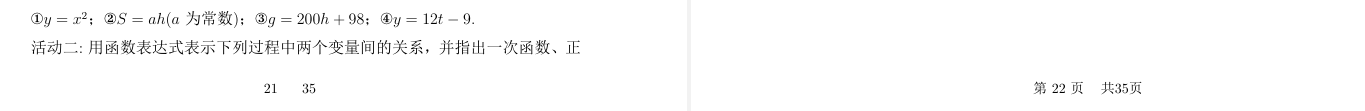
\includegraphics[width=\textwidth]{figure/chap-text/pifontconflict.png}
    \caption{页脚中文不显示}
\end{figure}

\qaq{解决方法:}参考\href{https://github.com/CTeX-org/ctex-kit/issues/688}{pifont宏包可能会触发中文不显示},把\lstinline{\makexeCJKactive}加到页眉页脚的开头。
\begin{lstlisting}
    \fancyfoot[C]{  \songti 第\thepage 页  \hspace{0.5em} 共\pageref{LastPage}页}
\end{lstlisting}

\section{脚注}\label{sec:footnote}

脚注命令:
\begin{lstlisting}
\footnote[手动指定序号,可忽略]{脚注内容}
\end{lstlisting}



\section{尾注}\label{sec:endnote}
\LaTeX{} 目前没有提供直接插入尾注的命令,但可以调用endnotes宏包实现。

不常用,暂时略过。

\section{交叉引用}\label{sec:crossref}
可以使用\lstinline|\ref|命令和\lstinline|\label|命令进行交叉引用。在正文中,使用\lstinline|\ref{label}|命令引用,在相应位置使用\lstinline|\label{label}|命令进行标记。

\section{列表}\label{sec:list}

\subsection{无序列表}\label{subsec:itemize}
无序列表环境:

\vspace{2em}
\begin{minipage}{0.45\textwidth}
    \begin{lstlisting}
        \begin{itemize}
            \item 第一项
            \item [-]第二项
            \item [*]第三项
        \end{itemize}
    \end{lstlisting}
\end{minipage}
\begin{minipage}{0.45\textwidth}
    \begin{itemize}
        \item 第一项
        \item [-]第二项
        \item [*]第三项
    \end{itemize}
\end{minipage}

条目之间间距较大,可以使用长度赋值命令将条目环境额外的垂直空白设置为0pt,达到与正文间距一致:

\begin{lstlisting}
    \itemsep=0pt
    \parskip=0pt
\end{lstlisting}


\subsection{有序列表}\label{subsec:enumerate}
有序列表环境:

\vspace{2em}
\begin{minipage}{0.45\textwidth}
    \begin{lstlisting}
        \begin{enumerate}
            \item 第一项
            \item 第二项
            \item 第三项
        \end{enumerate}
    \end{lstlisting}
\end{minipage}
\begin{minipage}{0.45\textwidth}
    \begin{enumerate}
        \item 第一项
        \item 第二项
        \item 第三项
    \end{enumerate}
\end{minipage}

有序列表可以嵌套,可对其序号、标号和前缀进行重定义,但是比较麻烦,可以使用paralist宏包。


\subsection{paralist宏包}\label{subsec:paralist}

暂未接触使用,略过。

\section{代码展示}\label{sec:codeshow}

因为\LaTeX{}排版会自动忽略空白字符等,如果需要按照原格式排版,可以使用\lstinline{verbatim}环境。


\begin{codeshow}
    不使用verbatim环境:
    int main() {
            printf("Hello, world!");
            return 0;
        }

    使用verbatim环境:
    \begin{verbatim}
        int main() {
            printf("Hello, world!");
            return 0;
        }
    \end{verbatim}
\end{codeshow}

行内可以使用\lstinline{\verb|内容|}。

也可以使用\lstinline{lstlisting}宏包。可以实现复杂的高亮效果,但需要额外的配置。

% !TEX root = ../latexnote.tex
\chapter{图片}\label{chap:figure}
\section{简述}\label{sec:figure-intro}
\LaTeX{} 本身不支持插图功能,需要借助graphicx宏包。

使用 latex + dvipdfmx 编译命令时,调用 graphicx 宏包时要指定 dvipdfmx 选项\footnote{早期常使用 latex + dvips 组合命令,后者将 .dvi 文件转为 .ps 文件(PostScript),可进一步通过 ps2pdf 工具生成 PDF。dvips 和 dvipdfmx 在图形、颜色、超链接等功能的实现上有差别,而 \LaTeX{} 无法识别用户是用 dvips 还是dvipdfmx,所以要指定选项(缺省为 dvips)。};而使用 pdflatex 或 xelatex 命令编译时不需要。

下表给出了不同编译命令支持的图片格式:

\begin{table}[htp]
    \centering
    \caption{各种编译方式支持的主流图片格式}\label{tbl:figure-format}
    \begin{tabular}{*{3}{l}}
        \hline
        \textbf{格式}              & \textbf{矢量图} & \textbf{位图}      \\
        \hline
        {latex + dvipdfmx}       & {.eps}       & N/A              \\
        \quad (调用 {bmpsize} 宏包 ) & {.eps .pdf}  & {.jpg .png .bmp} \\[.3\baselineskip]
        {pdflatex}               & {.pdf}       & {.jpg .png}      \\
        \quad (调用 {epstopdf} 宏包) & {.pdf .eps}  & {.jpg .png}      \\[.3\baselineskip]
        {xelatex}                & {.pdf .eps}  & {.jpg .png .bmp} \\
        \hline
    \end{tabular}
    \begin{quote}\footnotesize
        注:在较新的 \TeX{} 发行版中,{latex + dvipdfmx} 和 {pdf\-latex} 命令可不依赖宏包,支持原来需要宏包扩展的图片格式
        (但 {pdf\-latex} 命令仍不支持 {.bmp} 格式的位图)。
    \end{quote}
\end{table}

引入graphicx 宏包后,可使用 \lstinline|\includegraphics| 命令插入图片,其语法为:


\begin{lstlisting}
\includegraphics[options]{file} % options可指定图片属性,如width=
\end{lstlisting}


其中,options 可选参数有:

\begin{table}[htp]
    \centering
    \caption{ \lstinline{\includegraphics} 命令的可选参数}\label{tbl:graphics-options}
    \begin{tabular}{lp{18em}}
        \hline
        \textbf{参数}     & \textbf{含义}          \\
        \hline
        width={width}   & 将图片缩放到宽度为{width}     \\
        height={height} & 将图片缩放到高度为{height}    \\
        scale={scale}   & 将图片相对于原尺寸缩放{scale} 倍 \\
        angle={angle}   & 将图片逆时针旋转{angle} 度    \\
        \hline
    \end{tabular}
\end{table}

\section{浮动体}\label{sec:figure-float}

浮动体将图、表与其标题定义为整体,然后动态排版,以解决图、表卡在换页处造成的过长的垂直空白的问题。图片的浮动体是figure。

下面是一个例子:
\begin{lstlisting}
\begin{figure}[htbp]
    \centering
    \includegraphics[width=0.8\textwidth]{example-image}
    \caption{This is an example image.}
    \label{fig:example-image}
\end{figure}
\end{lstlisting}

参数htbp表示浮动体的位置,h表示插入此处、t表示在页面上端,b表示在页面下端、p表示允许浮动体单开一页。

% !TEX root = ../latexnote.tex
\chapter{表格}\label{chap:table}

\section{基本表格}\label{sec:basic-table}

表格和图片类似,也有一个浮动体环境为table。

表格最基本的环境为tabular,用法如下:
\begin{lstlisting}
\begin{tabular}[可选参数]{|c|c|c|}
\hline
第一列 & 第二列 & 第三列 \\
\hline
1 & 2 & 3 \\
4 & 5 & 6 \\
\hline
\end{tabular}
\end{lstlisting}

其中\lstinline{|c|c|c|}是列格式标记,详细见\ref{sec:liegeshi},c表示列居中,|表示列之间有竖线。使用\&用来分割列,使用\lstinline|\\|表示换行。\lstinline{\hline}用来绘制行之间的横线。

\subsection{修改表格线}\label{sec:modify-table-line}
可在tabular环境外修改全部表格线的粗细,如\lstinline|\setlength{\arrayrulewidth}{2pt}|或\lstinline{\arrayrulewidth=2pt}。

如果需要单独修改表格线,可采用如下方法:

1)修改垂直表格线,使用array宏包提供的新列格式选项定义命令:
\begin{lstlisting}
\newcolumntype{新选项名称}[参数数量]{列格式}
\newcolumntype{I}{!{\vrule width 2pt}}
\end{lstlisting}
\begin{codeshow}
    \centering
    \newcolumntype{I}{!{\vrule width 2pt}}
    \begin{tabular}{|cIcIc|}
        \hline
        \multicolumn{3}{IcI}{垂直线粗细更改} \\
        \hline
        7 & 5 & 3                     \\
        \hline
        6 & 1 & 8                     \\
        \hline
    \end{tabular}
\end{codeshow}

2)修改水平表格线,可使用booktabs宏包,该宏包可以任意修改水平线粗细,还可以在上下附加一段垂直空白。

\begin{codeshow}
    \centering
    \begin{tabular}{|c|c|c|}
        \hline
        \multicolumn{3}{|c|}{水平表格线粗细更改} \\
        \specialrule{2pt}{0pt}{0pt}
        7 & 5 & 3                       \\
        \hline
        6 & 1 & 8                       \\
        \hline
    \end{tabular}
\end{codeshow}

\subsection{列格式}\label{sec:column-format}
\label{sec:liegeshi}

基本列格式如下表所示:

\begin{table}[htp]
    \centering
    \caption{\LaTeX{} 表格列格式}\label{tbl:table-column-spec}
    \begin{tabular}{*{2}{l}}
        \hline
        \textbf{列格式} & \textbf{说明}            \\
        \hline
        l/c/r        & 单元格内容左对齐/居中/右对齐,不折行    \\
        p\{width\}   & 单元格宽度固定为 {width},可自动折行 \\
        |            & 绘制竖线                   \\
        @\{string\}  & 自定义内容 {string}         \\
        \hline
    \end{tabular}
\end{table}

格中每行的单元格数目不能多于列格式里 l/c/r/p 的总数(可以少于这个总数),否则出错。

@ 格式可在单元格前后插入任意的文本,但同时它也消除了单元格前后额外添加的间距。@格式可以适当使用以充当“竖线”。特别地,\lstinline|@{}| 可直接用来消除单元格前后的间距。

另外\LaTeX{} 还提供了简便的将格式参数重复的写法 \lstinline|*{⟨n⟩}{⟨column-spec⟩}|,比如以下两种写法是等效的:
\begin{lstlisting}
    \begin{tabular}{|c|c|c|c|c|p{4em}|p{4em}|}
    \begin{tabular}{|*{5}{c|}*{2}{p{4em}|}}
\end{lstlisting}


\subsection{列宽}\label{sec:column-width}

\LaTeX{} 本身提供了 tabular* 环境用来排版定宽表格,但是不太方便使用,比如要用到 @ 格式插入额外命令,令单元格之间的间距为 \lstinline{\fill},但即使这样仍然有瑕疵:

\begin{codeshow}
    \begin{tabular*}{14em}%
        {@{\extracolsep{\fill}}|c|c|c|c|}
        \hline
        A & B & C & D \\ \hline
        a & b & c & d \\ \hline
    \end{tabular*}
\end{codeshow}

tabularx 宏包为我们提供了方便的解决方案。它引入了一个 X 列格式,类似 p 列格式,不过会根据表格宽度自动计算列宽,多个 X 列格式平均分配列宽。X 列格式也可以用 array 里的辅助格式修饰对齐方式:

\begin{codeshow}
    % \usepackage{array,tabularx}
    \begin{tabularx}{14em}%
        {|*{4}{>{\centering\arraybackslash}X|}}
        \hline
        A & B & C & D \\ \hline
        a & b & c & d \\ \hline
    \end{tabularx}
\end{codeshow}

\subsection{行距}\label{sec:row-spacing}

修改参数 \lstinline{\arraystretch} 可以得到行距更加宽松的表格:
\begin{lstlisting}
    \renewcommand\arraystretch{1.8}
\end{lstlisting}

另一种增加间距的办法是给换行命令 \lstinline|\\| 添加可选参数,在这一行下面加额外的间距,适合用于在行间不加横线的表格:


\subsection{表格标题}\label{sec:table-title}

表格标题可以用\lstinline{\caption}命令设置,默认只能在浮动体环境内部使用。

也可以在导言区添加如下命令,在浮动体外使用\lstinline{\figcaption}和\lstinline{\tabcaption}为图表添加标题。为了防止标题和图表不在一页,可以使用minipage环境将它们包起来。

\begin{lstlisting}
    \makeatletter
    \newcommand\figcaption{def\@captype{figure}\caption}
    \newcommand\tabcaption{def\@captype{table}\caption}
    \makeatother
\end{lstlisting}



\section{复杂表格}\label{sec:complex-table}

\subsection{合并单元格}\label{sec:merge-cell}

1)跨列

使用\lstinline{\multicolumn}命令可以合并列:
\begin{lstlisting}
    \multicolumn{合并列数目}{列格式}{内容}
\end{lstlisting}

2)跨行

跨行需要引入multirow宏包,使用\lstinline{\multirow}命令:
\begin{lstlisting}
    \multirow{合并行数目}{宽度}{内容} %宽度可以填*以使用自然宽度
\end{lstlisting}

既跨行又跨列时,需要把\lstinline{\multirow}命令放在\lstinline{\multicolumn}命令内部。

\begin{codeshow}
    \centering
    \begin{center}
        \begin{tabular}{|c|c|c|}
            \hline
            \multirow{2}{2cm}{A Text!}
                                     & ABC & DEF \\
            \cline{2-3}              & abc & def \\
            \hline
            \multicolumn{2}{|c|}
            {\multirow{2}*{Nothing}} & XYZ       \\
            \multicolumn{2}{|c|}{}   & xyz       \\
            \hline
        \end{tabular}
    \end{center}
\end{codeshow}

\section{问题}

\subsection{longtable与arydshln宏包冲突}\label{subsec:longtable-arydshln-conflict}
\qaq{问题:}最近帮人debug,使用longtable排版报错。
\begin{figure}[!h]
    \centering
    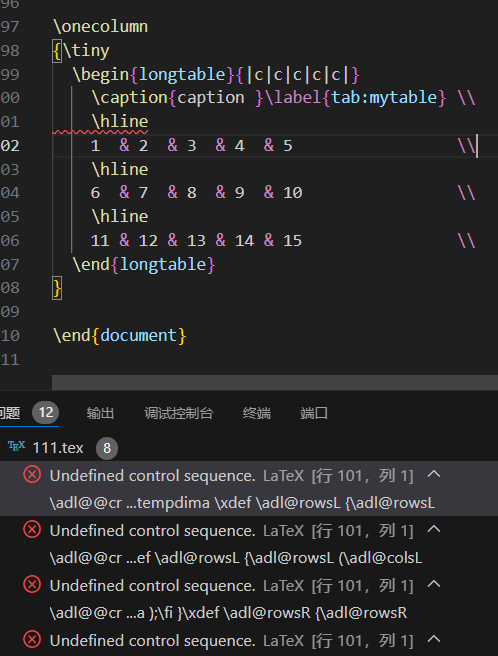
\includegraphics[width=0.4\textwidth]{figure/chap-tab/ary1.png}
    \caption{报错信息}
\end{figure}

\qaq{解决方法:}参考\href{https://zhuanlan.zhihu.com/p/667681242}{LaTeX:arydshln与longtable的冲突及教训 - 知乎 (zhihu.com)}, 发现longtable与arydshln宏包存在冲突,arydshln宏包重定义了\lstinline{\hline},可以采用如下解决方法:
\begin{enumerate}
    \item 注释掉\lstinline|\usepackage{arydshln}|。
    \item 将\lstinline|\usepackage{arydshln}|放于\lstinline|\usepackage{longtable}|之后
\end{enumerate}

\subsection{cline命令 undefined control sequence报错}\label{subsec:cline-undefined-control-sequence-error}
\qaq{问题:}使用Springer模板制作表格,使用\lstinline{\cline}命令报错,提示\lstinline{undefined control sequence}。

\qaq{解决方法:}Springer模板重新定义了\lstinline{\cline}命令,找到Springer模板的\lstinline{sn-jnl.cls}文件,将下面一行注释掉:
\begin{lstlisting}
    \let\cline\cmidrule
\end{lstlisting}

\subsection{multirow宏包居中}\label{subsec:multirow-center}

\qaq{问题:}列格式设置为居中,但是使用multirow多行合并内容不会居中

\qaq{解决方法:}添加如下命令:
\begin{lstlisting}
\renewcommand{\multirowsetup}{\centering}
\end{lstlisting}

% !TEX root = ../latexnote.tex
\chapter{数学公式}\label{chap:math}
\section{行内公式}\label{sec:inline}
行内公式使用\lstinline|\$|和\lstinline|\$|包裹,如:

\begin{codeshow}
    行内公式测试$a=b$
\end{codeshow}

\section{行间公式}\label{sec:display}
行间公式使用\lstinline|\begin{equation}|和\lstinline|\end{equation}|包裹,如:

\begin{codeshow}
    \begin{equation}
        a+b=c
    \end{equation}
\end{codeshow}

使用\lstinline|\begin{equation*}|和\lstinline|\end{equation*}|包裹的公式不带编号,如:

\begin{codeshow}
    \begin{equation*}
        a+b=c
    \end{equation*}
\end{codeshow}
% !TEX root = ../latexnote.tex
\chapter{参考文献设置}\label{chap:ref}
\section{问题}

\subsection{不按出现顺序引用}\label{subsec:not-in-order}
\qaq{问题:}Latex中ACM-Reference-Format顺序与论文引用顺序不一致

\qaq{解决方法:}修改\textcolor{red}{\lstinline{ACM-Reference-Format.bst}}文件,将大写SORT注释掉,一共两处。

\subsection{作者年份引用设置仅年份超链接}\label{subsec:year-only}
\qaq{问题:}Latex中采用作者年份引用,默认作者和年份都出现超链接,设置仅年份出现超链接

\qaq{解决方法:}在\lstinline|\begin{document}|前加入如下代码:
\begin{lstlisting}
\makeatletter
% Patch case where name and year are separated by aysep
\patchcmd{\NAT@citex}
  {\@citea\NAT@hyper@{%
     \NAT@nmfmt{\NAT@nm}%
     \hyper@natlinkbreak{\NAT@aysep\NAT@spacechar}{\@citeb\@extra@b@citeb}%
     \NAT@date}}
  {\@citea\NAT@nmfmt{\NAT@nm}%
   \NAT@aysep\NAT@spacechar\NAT@hyper@{\NAT@date}}{}{}

% Patch case where name and year are separated by opening bracket
\patchcmd{\NAT@citex}
  {\@citea\NAT@hyper@{%
     \NAT@nmfmt{\NAT@nm}%
     \hyper@natlinkbreak{\NAT@spacechar\NAT@@open\if*#1*\else#1\NAT@spacechar\fi}%
       {\@citeb\@extra@b@citeb}%
     \NAT@date}}
  {\@citea\NAT@nmfmt{\NAT@nm}%
   \NAT@spacechar\NAT@@open\if*#1*\else#1\NAT@spacechar\fi\NAT@hyper@{\NAT@date}}
  {}{}

\makeatother
\end{lstlisting}

\subsection{作者年份引用设置et al为斜体}\label{subsec:et-al-italic}
\qaq{问题:}Latex中采用作者年份引用,设置et al为斜体

\qaq{解决方法:}在相应\textcolor{red}{\lstinline|.bst|}文件中将\textcolor{red}{\lstinline{et~al.}}修改为\textcolor{red}{\lstinline|\\textit{et~al.}|},不要修改\textcolor{red}{\lstinline{et al}}

\subsection{beamer参考文献断行}\label{subsec:beamer-ref-break}
\qaq{问题:}beamer参考文献断行显示,如图\ref{fig:beamer-ref}所示。
\begin{figure}[!h]
  \centering
  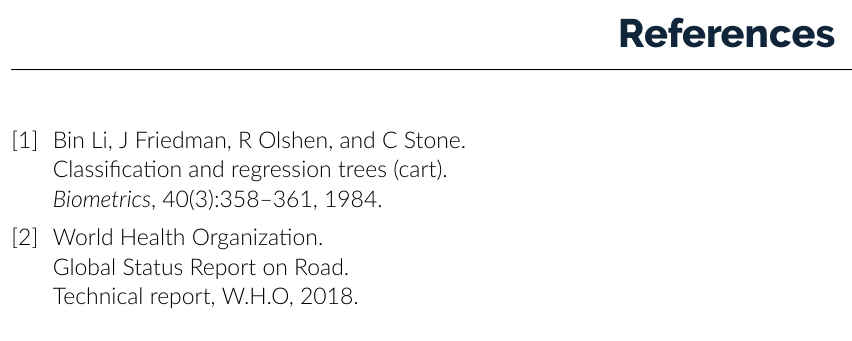
\includegraphics[width=0.8\textwidth]{figure/chap-ref/cankaowenxianduanhang.png}
  \caption{beamer参考文献断行显示}
  \label{fig:beamer-ref}
\end{figure}

\qaq{解决方法:}在导言区加入如下代码:
\begin{lstlisting}
  \setbeamertemplate{bibliography entry title}{}
  \setbeamertemplate{bibliography entry location}{}
  \setbeamertemplate{bibliography entry note}{}
\end{lstlisting}
\begin{figure}[!h]
  \centering
  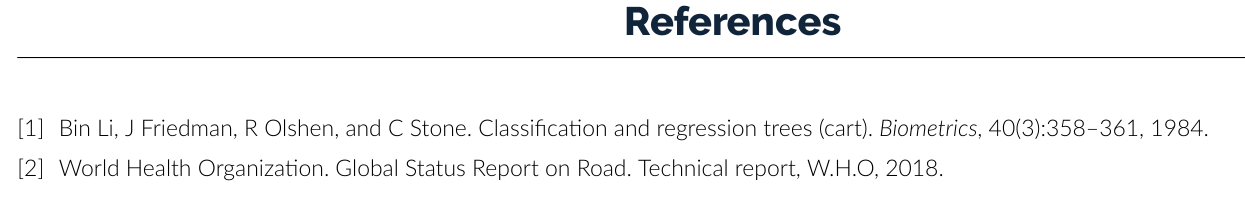
\includegraphics[width=0.8\textwidth]{figure/chap-ref/cankaowenxianduanhang1.png}
  \caption{beamer参考文献正常显示}
  \label{fig:beamer-ref1}
\end{figure}
% !TEX root = ../latexnote.tex

% !TEX root = ../latexnote.tex
\chapter*{参考资料}\label{chap:refinfor}
\addcontentsline{toc}{chapter}{参考资料}
\begin{enumerate}[itemsep=1.5ex]
    \item \href{https://zhuanlan.zhihu.com/p/248669482}{TeX 家族(TeX, XeTeX, LuaTeX,XeLaTeX …看完这篇就懂了)}
    \item \href{http://mirrors.ctan.org/info/lshort/chinese/lshort-zh-cn.pdf}{一份(不太)简短的 \LaTeX{}2$\epsilon$介绍}
    \item \href{https://github.com/zousiyu1995/Study-LaTeX}{邹思宇的\LaTeX{}2$\epsilon$学习笔记}
    \item \href{https://blog.csdn.net/qq_36829039/article/details/123576507}{参考文献全超链接+仅年份超链接\_latex 参考文献仅年份超链接-CSDN博客}
    \item \href{https://tex.stackexchange.com/questions/532367/bibtex-style-with-et-al-in-italic}{BibTeX style with "et al" in italic - TeX - LaTeX Stack Exchange}
    \item \href{https://zhuanlan.zhihu.com/p/667681242}{LaTeX:arydshln与longtable的冲突及教训 - 知乎 (zhihu.com)}
    \item \href{https://syvshc.github.io/2021-04-07-illegal-temp-cause-tlinstall-failure/}{Windows 不合法的缓存路径导致 TeX Live 安装失败}
    \item \href{https://github.com/CTeX-org/ctex-kit/issues/688}{pifont宏包可能会触发中文不显示}
\end{enumerate}

% \printbibliography[heading=bibintoc, title=\ebibname]

%附录
\appendix

\end{document}
